\documentclass[runningheads,a4paper]{llncs}
\usepackage{amssymb}
\setcounter{tocdepth}{3}
\usepackage{graphicx}

\begin{document}

\mainmatter  % start of an individual contribution
\title{Integrated Optimization Methodology for Data Interleaving and Memory Mapping on VLIW architectures}
\titlerunning{Interleaving and mapping co-exploration}
\author{Draft}
%\author{Iason, Namita, Francky, PG, others}
%\institute{IMEC, ...}
\maketitle

\begin{abstract}
This work presents a methodology for efficient exploration of data interleaving and data-to-memory mapping options for SIMD platform architectures, which include VLIW function units and a reconfigurable clustered memory. 
The scope is the reduction of the overall energy consumption by increasing the utilization of FUs and decreasing the number of memory accesses.
The presented methodology is tested using a number of benchmark applications with irregularities on their access scheme.
Potential gains are calculated based on energy models both for the processing and the memory part of the system.

\end{abstract}

\section{Introduction}

The goal of this work is to improve both the performance and the energy consumption for data intensive applications. 
We focus on SIMD architectures and deal with applications that have irregularities on their access scheme. 
SIMD architectures can potentially increase the performance of an application, providing that the utilization of them is high. 
However, applications with irregular access patterns do not provide compact sequences of data that are suitable for high utilization. 
Hence the performance is lower than expected. 
In order to improve the performance a systematic exploration of the interleaving options for application's data is needed. 

The energy consumption can be divided into two parts, namely the processing and the memory subsystem. 
The energy needed for processing depends mainly on the utilization of the FUs and any potential stalls, if the memory cannot provide data on the needed rate.
The interleaving exploration can increase the utilization of the processing subsystem and reduce time penalties for data loading.   
The energy consumption on the memory subsystem is affected by the number of memory accesses and the energy per access. 
Again, the memory architecture and the data-to-memory mapping decisions have a great impact on both the number of accesses and the energy per access.

%\section{Related work}

\section{System Design Exploration Workflow}

The general workflow of this work is presented in Fig.\ref{workflow}.

\begin{figure}
\centering
	\label{workflow}
	\caption{Methodology steps}
	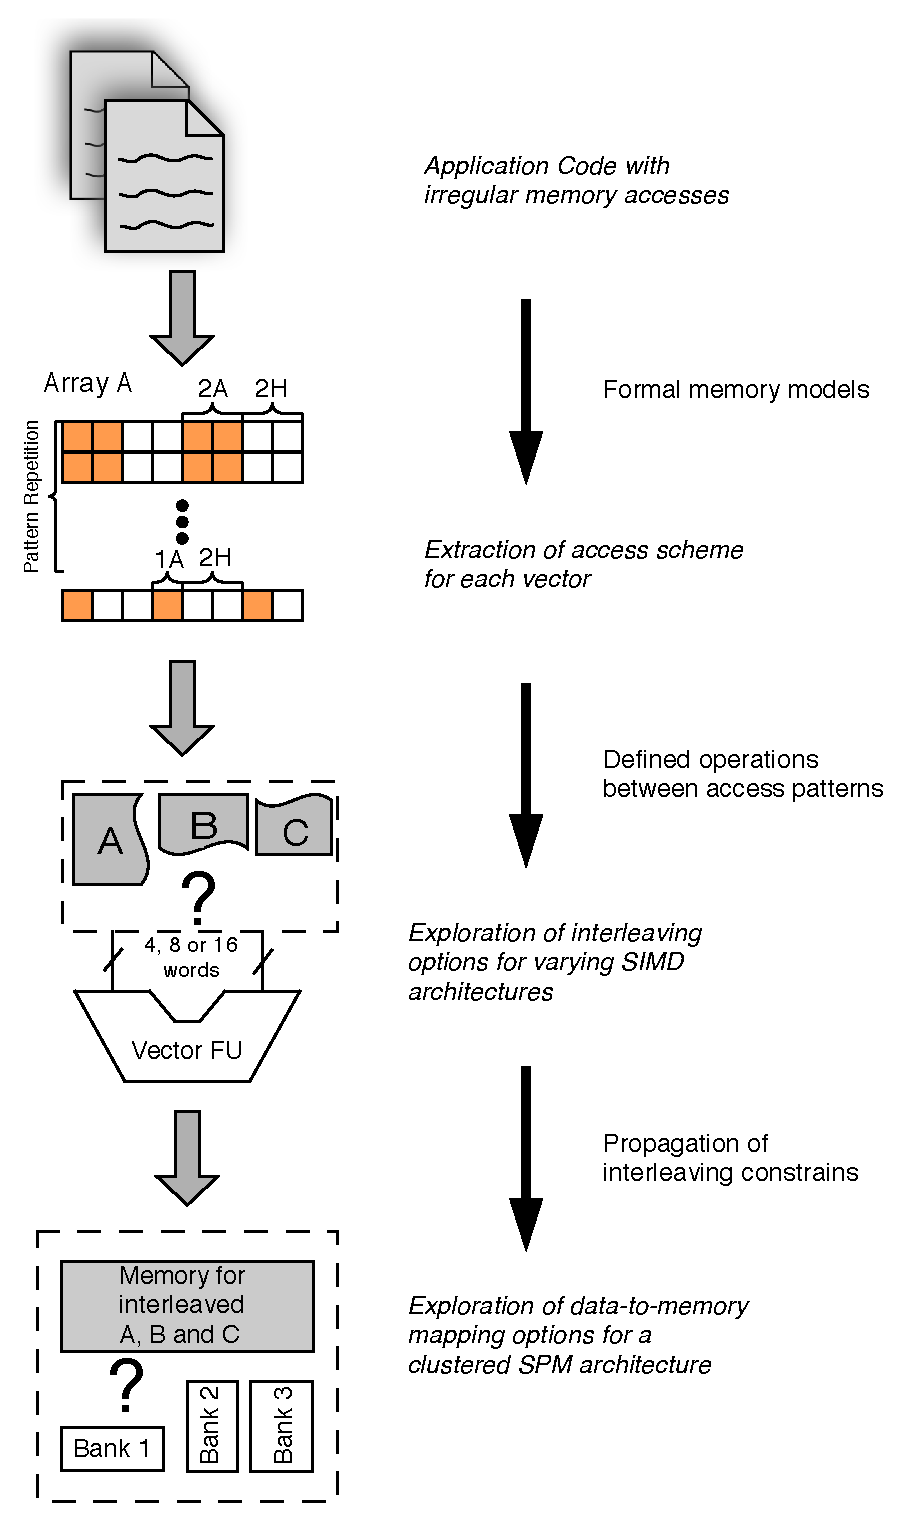
\includegraphics[width=\textwidth]{Images/Workflow.eps} 
\end{figure}

\subsection{Formal Model Representation of Access Pattern }

A representation model for the access pattern is employed in order to formally present each step of the methodology.

\textit{Discussion about polyhedral and enumerative approaches}

\textit{Analysis of A-H model based on Angeliki}

\textit{Definition of algebra functions between access patterns}

\subsection{Data Interleaving Exploration}

\textit{Algorithm for exploring data interleaving}

\subsection{Data-to-Memory Mapping Exploration}

Given the input from the previous step, we explore the mapping of data-to-memory.

\subsection{One way constraint propagation}

The decisions taken on the interleaving step affect the mapping options.
If the interleaving decisions lead to small compact sets of data, the mapping can be done on small energy efficient memory banks.
On the other hand, if the mapping exploration is performed first, the freedom for interleaving is reduced.
We split the decisions in two steps and the interleaving decisions are propagated as constraints on the mapping exploration phase. 

\section{Target Architecture}

\textit{Analysis of architecture based on our previous papers}

General architecture is presented in Fig.\ref{arch}.

\begin{figure}
\centering
	\label{arch}
	\caption{Exploration options and system knobs depending on a general platform architecture}
	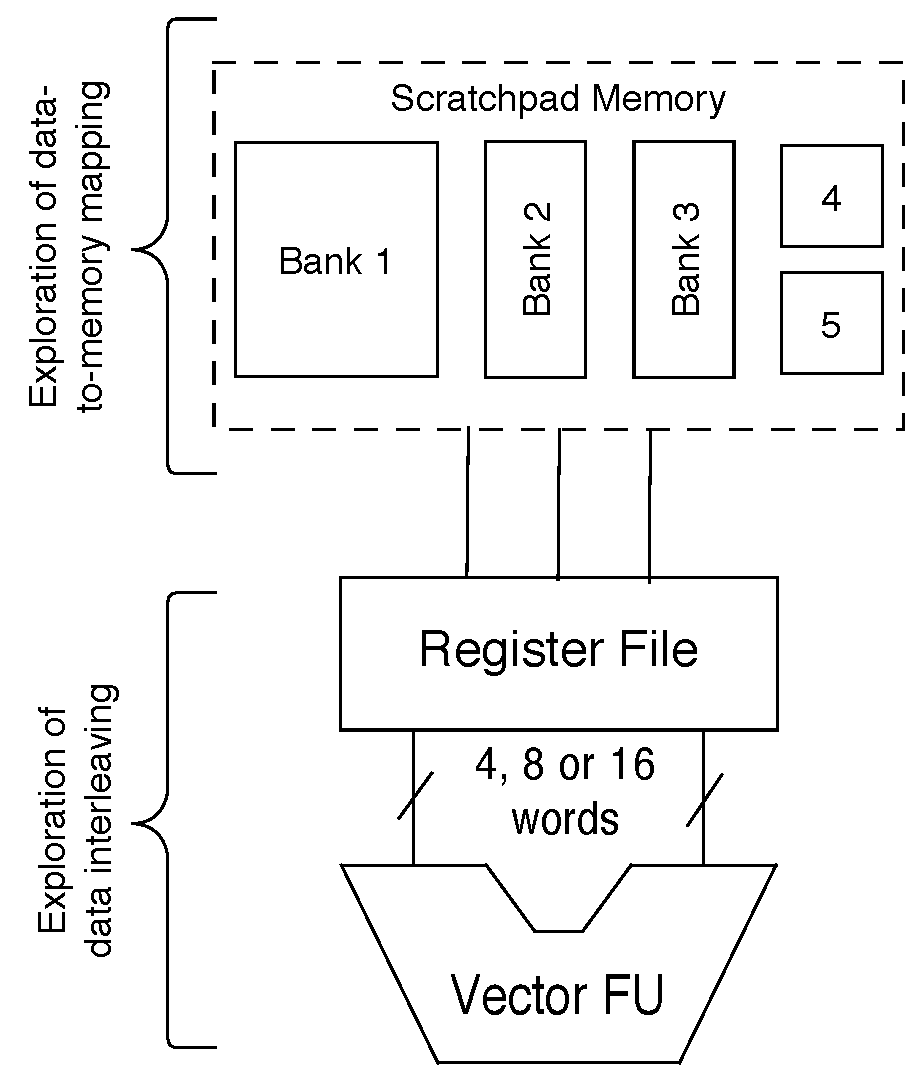
\includegraphics[width=\textwidth]{Images/Architecture.eps} 
\end{figure}

\section{Applications}

An example of the channel estimation kernel is presented in Fig.\ref{example}.

\begin{figure}
\centering
	\label{example}
	\caption{Exploration example for the channel estimation kernel}
	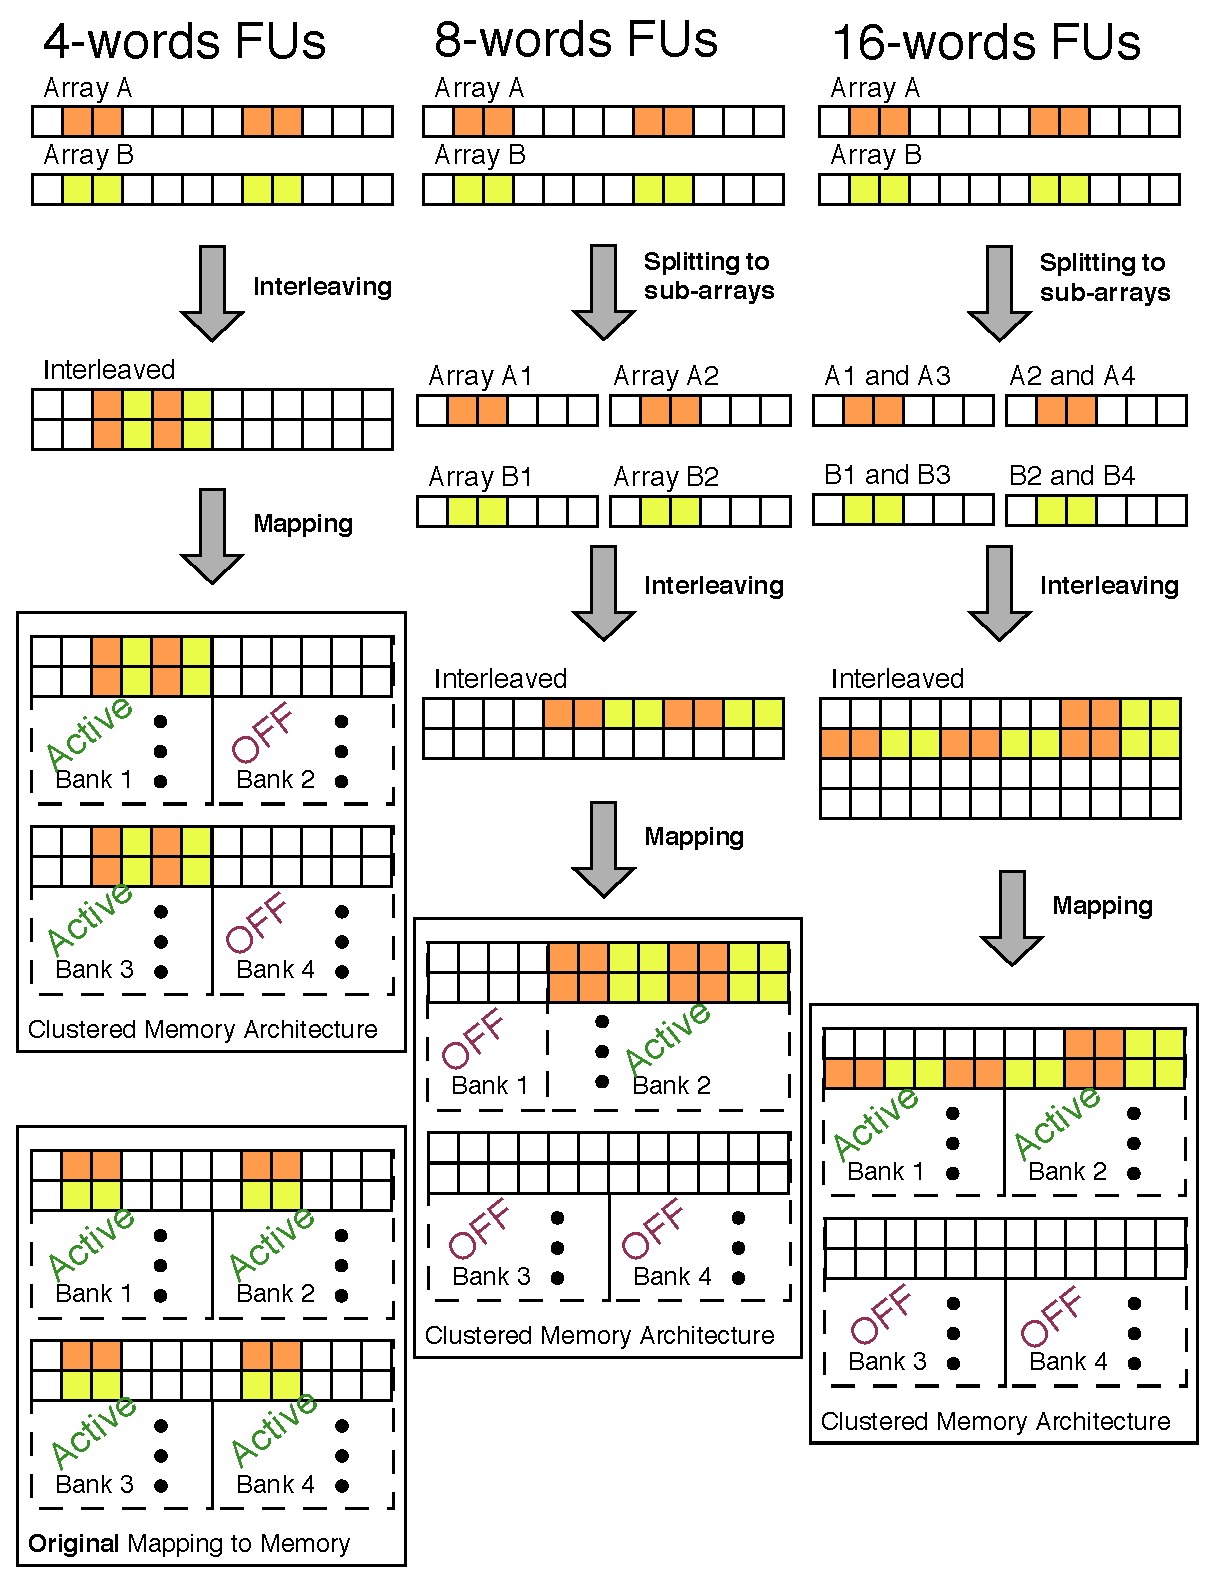
\includegraphics[width=\textwidth]{Images/Example.eps} 
\end{figure}

Suitable applications:
\begin{itemize}
\item Channel estimation kernel
\item SOR benchmark
\item Motion estimation kernel
\item PGM-armor
\item Maybe image processing...
\end{itemize}

\section{Results}

The design exploration is applied to the chosen application benchmark and energy numbers are derived based on the described target platform.
Results are presented for the four cases:
\begin{itemize}
\item No optimization
\item Interleaving exploration with a static memory platform (gain A)
\item Data mapping exploration on a reconfigurable platform without optimized interleaving (gain B)
\item Co-exploration of interleaving and mapping options (gain C, C$ > $A+B )
\end{itemize}

\end{document}